\documentclass[]{article}
\usepackage{amsmath}
\usepackage{amssymb}
\usepackage{graphicx}

\title{Physics 229}
% \author[1]{Andrew MacRae}
% \affil[1]{D of P and A, U of V}
\begin{document}
\section{Amplifiers}
\subsection{Active vs. Passive Circuits}
We now move into the regime of so-called \textit{active electronics}. Everything studied so far -- resistors and capacitors, to voltage dividers and filters, to diode rectifiers has fallen under the realm of passive electronics. Active electronic devices, in addition to standard inputs and outputs, require additional power supplies in order to function. There are great benefits to this, as we shall see: active components can output more power than at their input, and can eliminate annoying effects such as voltage loading due to input and output impedance. The first active device we'll study is the amplifier.
\subsection{The Ideal Voltage Amplifier}
The idea of the basic amplifier is simple: take the input $x_\text{in}$ and produce an output which is some number $G$ times the output.
\begin{equation}
\label{eq:simple_amp}
x_\text{out} = Gx_\text{in}
\end{equation}

\noindent ... where $G$ is known as the gain.

There is the question of what input $x_\text{in}$ is being amplified. In our course, normally $x_\text{in}$ will be a voltage and so we will have a voltage amplifier. In this case the gain is often expressed in decibals as:

\begin{equation}
\label{eq:voltage_amp_dB}
G_\text{dB} = 20\log\frac{v_\text{out}}{v_\text{in}} 
\end{equation}

We will occasionally deal with power amplifiers whose input and output is a power. For these amplifiers, the gain is also in dB but with a 10 instead of a 20 multiplier\footnote{Recall that for a fixed load resistance, $P = v^2/R \propto v^2$. Thus $10\log\left[P_\text{out}/P\text{in}\right] = 10\log\left[\left(v_\text{out}/v\text{in}\right)^2\right] = 20\log\left[v_\text{out}/v_\text{in}\right]$, thus yielding consistant definitions of gain}:

\begin{equation}
\label{eq:power_amp_dB}
G_\text{dB} = 10\log\frac{P_\text{out}}{P_\text{in}} 
\end{equation}

\noindent For now though, we will restrict outselves to voltage amplifiers. Diagrammed in figure \ref{fig:simple_amp}. The output is descibed by equation \ref{eq:simple_amp}.

\begin{figure}[h]
\caption{The simplest of amplifiers: the output is the input multiplied by a constant gain $G$.}
\label{fig:simple_amp}
\begin{center}
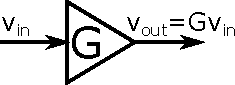
\includegraphics{Images/SimpleAmplifier.pdf}
\end{center}
\end{figure}

\subsection{Reality Check: Amplifiers in Real Life}
There are several limitations to the ideal amplifier that come into effect in practice. For example the amplifier will have to draw at least a small current from the source in order to operate. As we've learned, this is equivalent to a finite \textit{input impedance} $R_\text{in}$. The amplifier will also have a limit to how much current it can output due to its internal resistances. This leads to a finite \textit{output impedance} $R_{out}$. There are also limits to how fast the amplifier can respond to a changing input signal. This leads to a finite \textit{gain bandwidth}, or in general, a frequency dependant gain $G(\omega)$. We will examine each of these effects presently.

\subsubsection{Effects of Finite Input Impedance}
We can model the non-ideal amplifier as an ideal amplifier inside a black box, precisely as we did with ideal vs real voltage sources. Inside the black-box, the input impedance is models as an internal resistance $R_\text{in}$ to ground placed before the ideal amplifier. This forms a voltage divider with the input impedance from the rest of the circuit so that there is some voltage drop. The ideal amplifier thus sees a different voltage than $v_\text{in}$, which we denote $v^\prime_\text{in}$. The output of the real amplifier is thus less than we would expect: $v_\text{out} = Gv^\prime_\text{in} < Gv_\text{in}$
\begin{figure}[h]
\caption{We model the finite input impedance of the amplifier as a internal resistor $R_\text{in}$ to ground before an ideal amplifier all in a black box.}
\label{fig:real_amp_int}
\begin{center}
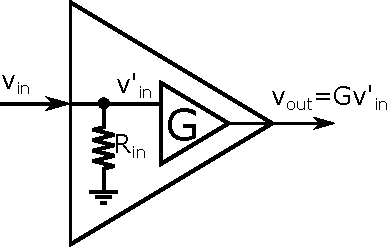
\includegraphics{Images/RealAmplifier_int.pdf}
\end{center}
\end{figure}

The true output, given the input impedance can be calculated given the output impedance of whatever follows. For example, with a $100$~$\Omega$ input impedance amplifier with $G = 10$, 

\subsubsection{Effects of Finite Output Impedance}
The operation of our ideal amplifier can be seen as a two part process: first it senses the voltage at its input (with the effect of finite input impedance causing some loading error), and second, it acts as a new voltage source, producing a voltage $v_\text{out} Gc_\text{in}$. As with any \textit{real} source, it will be equivalent to an ideal source, in series with an output impedance $R_\text{out}$. This finite output impedance leads to a maximum short-circuit current of $v_\text{out}/R_\text{out}$ and will lead to all of the loading issues discussed in chapter XXX. Figure \ref{fig:real_amp_int_out} shows our improved model of how a real amplifier behaves.
\begin{figure}[h]
\caption{A better model of a real amplifier has an input resistance to ground in parallel with the inpput and an output resistance in series with its output.}
\label{fig:real_amp_int_out}
\begin{center}
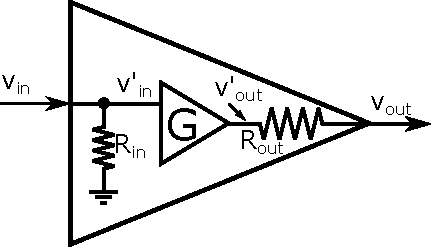
\includegraphics{Images/RealAmplifier_int_out.pdf}
\end{center}
\end{figure}

\noindent\textbf{Design Example:} Consider a real amplifier with $R_\text{in} = 10$~k$\Omega$, $R_\text{F} = 100~\Omega$, and G = 25. We use it to amplify a 10~mV signal from a photodetector having $R_\text{out,PD} = 1250~\Omega$ and send it to a (lousy) voltmeter with $R_\text{in,LVM}$ = 500~$\Omega$ (see figure \ref{fig:prob_amp}). What is the voltage measured (a) assuming an ideal $G = 25$ amplifier, and (b) with our real amplifier?\\\\\noindent Answer: For part (a) the answer is simply $v_\text{meas} = 25\times10~$mV = 250~mV. For our real amplifier, we must consider the input and output stage. The input now forms a voltage divider with $R_\text{in}$ (figure \ref{fig:prob_amp}b so that the inner ideal amplifier sees:
$$
v_\text{in}^\prime=\frac{R_\text{in}}{R_\text{out,PD} + R_\text{in}} = \frac{10~\text{k}\Omega}{11.25~\text{k}\Omega}\times10~\text{mV} \approx 8.9~\text{mV}
$$
In our model, this is then amplified by the ideal internal amplifier producing
$$
v_\text{out}^\prime = 8.9~\text{mV}\times 25 \approx 222~\text{mV}
$$
Finally, this is then sent to our lousy voltmeter, through its internal output resistance, forming another voltage divider (figure \ref{fig:prob_amp}c) to yeild the final voltage:
$$
v_\text{out} = \frac{R_\text{in,LVM}}{R_\text{out} + R_\text{in,LVM}}v_\text{out}^\prime = \frac{500~\Omega}{600~\Omega}\times 222~\text{mV}\approx 185~\text{mV}
$$

\begin{figure}[ht]
\caption{Example Problem.}
\label{fig:prob_amp}
\begin{center}
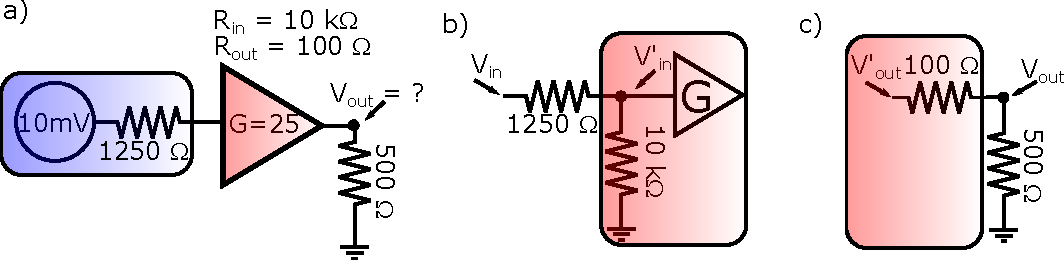
\includegraphics[width=\textwidth]{Images/amp_example.pdf}
\end{center}
\end{figure}

We thus see that the effect of finite input and output impedance is to lessen the effective gain of the real amplifier. Even if we used an ideal voltmeter with infinite input impedance, we'd still see 222~mV $<$ 250~mV. Equivalently, we could try to build an amplifier with $R_\text{out} \rightarrow 0~\Omega$ and again we'd see 222~mV, regardless of the impedance of the voltmeter. To get the full 250~mV however, we'd need to also have $R_\text{in} \rightarrow \infty$, so that $v_\text{in}^\prime = v_\text{in} = 25$~mV. 

From this we can infer the ideal characteristrics of a real amplifier: we want the input impedance as high as possible while having output impedance as low as possible. This can be accomplished using solid state transistors, discussed later in the course. 
\subsubsection{Effects of Finite Frequency Response}

\subsection{Effects of Noise: Noise Factor and SNR}

\subsection{Differential Amplifiers}

\subsection{Characterizing Differential Amplifier Performance: CMRR}
\subsubsection{Common Mode Gain}
\subsubsection{Common Mode Rejection Ratio}
\subsection{Special Purpose Amplifiers}
\subsubsection{Audio Amplifiers}
\subsubsection{Power Amplifiers}
\subsubsection{Instrumentation Amplifiers}
\subsubsection{Lock-In Amplifiers}
\end{document}